\begin{figure}[p]
\centering
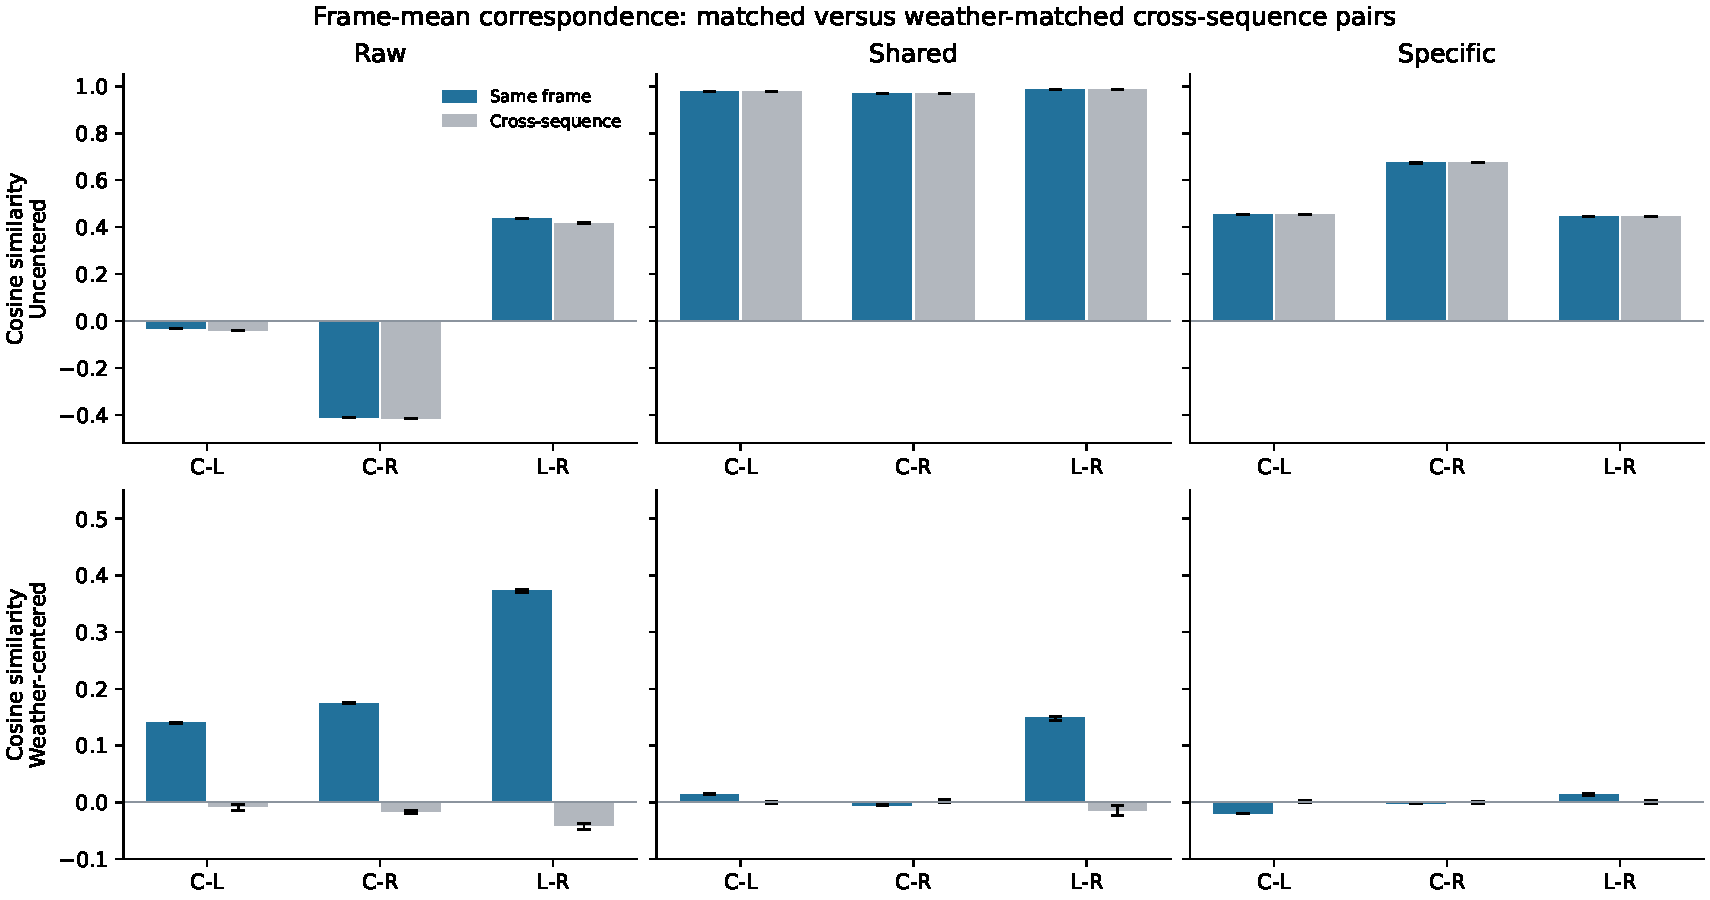
\includegraphics[width=\linewidth,height=.65\textheight,keepaspectratio]{assets/frame_correspondence.pdf}
\caption{Frame-level cross-modal correspondence controls using foreground-mean vectors in the original feature space. Same-frame pairs are compared with different-sequence pairs from the same weather group over ten fixed permutation seeds; matched scores use the same retained anchors. Weather-centered results subtract the mean for each modality, representation type, and weather group before computing cosine similarity. These are cosines of frame-mean vectors, unlike the averages of matched-patch cosines in Figure~\ref{fig:e2}. Seed variation concerns mismatch sampling, not independently trained models. High uncentered shared cosine persists under mismatching, so high similarity alone does not demonstrate semantic correspondence.}
\label{fig:e-correspondence}
\end{figure}
